\chapter{Theory}


\section{Wave Theory}

Simple Wave Theory

\section{Energy Spectra}

\subsection{Phillips Spectrum}
\subsection{Mobley Spectrum}
\subsection{SWAP}
\subsection{JONSWAP}


Energy Spectrum

$\int x(t) dt$

$k=\frac{\pi}{\mathbf y}$

\begin{equation}\label{eq:test} x = y \end{equation}

We can give an equation a label so that we can refer to it later.
\begin{equation}
\label{eq:ising}
E = -J \sum_{i=1}^N s_i s_{i+1} ,
\end{equation}
Equation~\eqref{eq:ising} expresses the energy of a configuration
of spins in the Ising model.

\section{The Rendering Pipeline}
%BLABLA
%
\begin{figure}[h]
\begin{center}

\includegraphics[scale=1.0]{Images/Rendering-Pipeline-AGR.pdf}
\end{center}
\end{figure}
\begin{figure}[t]
\begin{center}
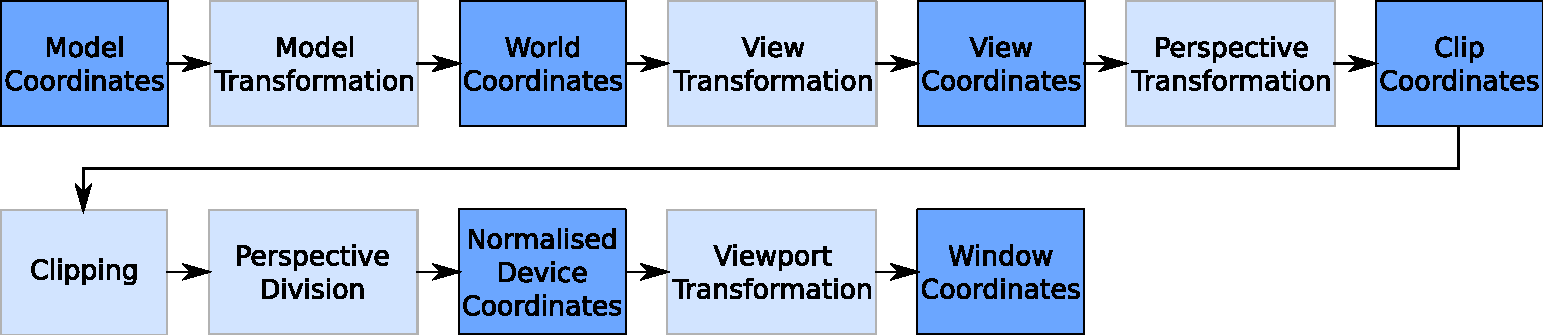
\includegraphics[scale=0.5]{Images/Geometry-Stage.pdf}
\end{center}
\end{figure}
%
%\begin{itemize}
% \item The \textit{application stage}
% \item The \textit{geometry stage}
% \item The \textit{rasterizer stage}
%\end{itemize}

\subsection{Application Stage}

software stage, excempt hardware accelerated physics and sound
holds high level scene information
prepares data to be processed by geometry stage

\subsection{Geometry Stage}

model coordinates
model matrix
world coordinates
view matrix
view coordinates
projection matrix
clip coordinates, cube
clipping
perspective division
normalized device coordinates
viewport transformation
window coordinates


\subsection{Rasterizer Stage}

triangle setup
scan conversion and interpolation
per fragment operations (texturing, ummadumshadern)

\section{The Projected Grid}

postprojection coordinates transformed to worldspace
grid on near and far plane, intersection with the y=0 plane
decouple projector from camera

\subsection{The Projector}
positioning
rotating
original is a hack, persistent grid mapping has a more stable approach
not optimal, because of "popping" at great distances
not so optimal distribution of the mesh resolution throughout worldspace
visual range issues
do some modifications to the mesh vertex distribution
reference to original paper from 2004 + persistent grid mapping

\section{Water optics}
BRAK

\section{Colour Management}

Explain color and gamma problem
linear vs nonlinear space

\subsection{gamma}
sRGB(gamma 2.2) support in hardware, convert from nonlinear space to linear
space do calculations on lighting and so on, back to srgb space
do tonemapping sRGB -> XYZ -> xyY -> modify Y -> XYZ -> sRGB

\subsection{device calibration}
short explanation of monitor calibration and so on
tools available


